\documentclass[conference]{IEEEtran}
\usepackage{algorithm}
\usepackage{algorithmic}
\usepackage{graphicx}
\usepackage{subfigure}
\usepackage{float}
\usepackage{amssymb}
\usepackage{amsmath}
\usepackage{textcomp}

\IEEEoverridecommandlockouts    
\textwidth 178mm    
\textheight 239mm  
\oddsidemargin -7mm
\evensidemargin -7mm
\topmargin -6mm
\columnsep 5mm

\begin{document}
\title{\ \\ \LARGE\bf Off-line handwritten word recognition using hidden Markov models}
\author{{\bf Davide Modolo} and {\bf Thijs Kooi}\\ Davide.Modolo@gmail.com\\ Thijs.Kooi@student.uva.nl}
\maketitle
\begin{abstract}
 
\end{abstract}

\section{Introduction}


\section{Pre-processing}
\section{Feature extraction}

In order to exploit the sequential nature of the data, we need a model that does not treat the data as i.i.d. This is provided by the {\it hidden Markov model}, a model widely used in the areas of speech recognition and language modelling. 
\section{Hidden Markov models}
%Work in progress!!!!
A Hidden Markov model is described by:
\begin{itemize}
 \item A set of $N$ states $S = (s_{1}, s_{2}, \ldots, s_{N})$, where the state of the system at time $t$ is denoted $q_{t}$
 \item A set of priors ${\bf \pi} = (\pi_{1}, \pi_{2}, \ldots, \pi_{N})$, providing the probability $P(q_{1} = s_{i})$.
 \item A transition function ${\bf A}$, where $a_{ij} = P(q_{j} = s_{j} | q_{i})$. 
 \item An observation function ${\bf B}$, mapping each observation at every state to a probability $b_{i}({\bf o}_{t}) = P({\bf o}_{t} | q_{t} = s_{i}, \lambda)$, where $\lambda$ denotes the model parameters.
\end{itemize}
The model is trained to estimate the posterior probability $P({\bf O}|\lambda)$ of an observation sequence ${\bf O}$, with $D$-dimensional observation vectors ${\bf o}_{t} = (o_{1},o_{2},\ldots,o_{D})$. We assume time to be discrete and the transition and observation probabilities to be static, i.e., they do not change over time. The hyperparameters we have to concern ourselves with are the network topology, i.e., the number of states and the transition probability and choise of the observation or emmision probability function. For speech and handwritten a left-to-right model is generally applied, as show in figure 1, though variations exist.\\
\begin{figure}[H]
 \centering
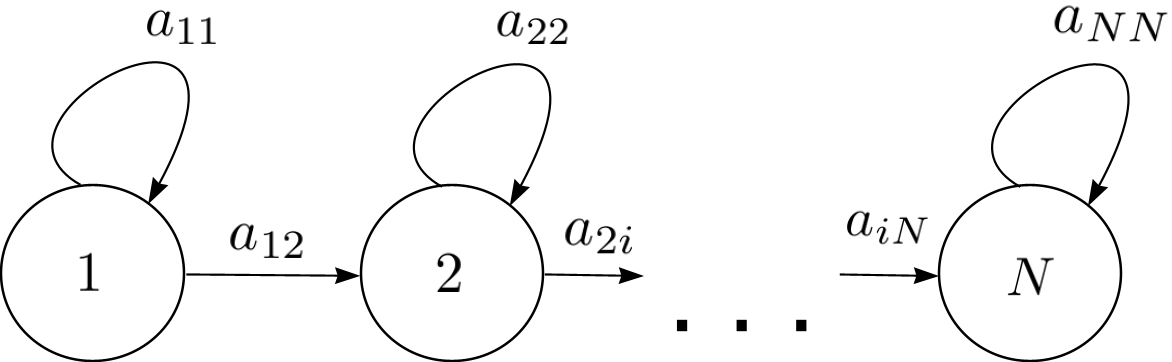
\includegraphics[width=0.35\textwidth]{hmm.jpg}
\caption{Illustration of a simple left-to-right model}
\end{figure}
The three main problems we want to solve for this model architecture are:
\begin{enumerate}
 \item The probability of an observation sequence, given the model, $P({\bf O}|\lambda)$.
 \item The most likely state sequence, underlying a given observation sequence and the model, $Q^* = \max P(Q|{\bf O},\lambda)$.
 \item The most likely parameters of the model $\lambda^* = \max P(X|\lambda)$, given a training set of $M$ observation sequences $X = ({\bf O}_{1}, {\bf O}_{2}, \ldots, {\bf O}_{M} )$.
\end{enumerate}
Probability of a state sequence $Q$, under the model $\lambda$:
\begin{equation}
 P(Q|\lambda) = \pi_{q_{1}}a_{q_{1}q_{2}} a_{q_{2}q_{3}} \ldots a_{q_{T-1}q_{T}}
\end{equation}

Probability of an observation sequence $O$, given a state sequence $Q$ and the model $\lambda$:
\[
 P({\bf O}|Q,\lambda) = P({\bf o}_{1}|q_{1})P({\bf o}_{2}|q_{2})\ldots P({\bf o}_{T}|q_{T}) =
\]
\begin{equation}
  b_{1}(o_{1})b_{2}(o_{2}) \ldots b_{T}(o_{T}) = \prod_{t = 1}^{T}b_{t}(o_{t})
\end{equation}
By the identity $P(A,B) = P(A|B)P(B)$, we have that:
\[
 P({\bf O},Q|\lambda) = P(O|Q,\lambda)P(Q|\lambda) = 
\]
\[
 \big[ \prod_{t = 1}^{T}b_{t}({\bf o}_{t}) \big] \pi_{q_{1}} \prod_{t = 1}^{T} a_{q_{t-1}q_{t}} =
\]
\[
 \pi_{q_{1}} b_{i}({\bf o}_{1}) \prod_{t = 2}^{T} a_{q_{t-1}q_{t}}b_{t}({\bf o}_{t})
\]
With the probability $P({\bf O}|\lambda)$ calculated by marginalising over all possible state sequences $Q$:
\[
 P({\bf O}|\lambda) = \displaystyle \sum_{Q} P({\bf O}|Q,\lambda)P(Q|\lambda) = 
\]
\begin{equation}
 \displaystyle \sum_{Q} \big[ \pi_{q_{1}} b_{q_{1}} \prod_{t=2}^{T} a_{q_{t-1}q_{t}}b_{q_{t}}({\bf o}_{t}) \big]
\end{equation}
A naive way to estimate the posterior of an observation sequence, would be to simply try all possible state sequences and evaluate their probability. Unfortunately, the number of state sequences increases exponentially with the number of observations, rendering the method $\mathcal{O}(N^{T})$ and thereby infeasable for all but the smallest models. Luckily, an alternative exists in the form of the {\it forward-backward} algorithm, a special instance of the {\it sum-product} algorithm.
\subsection{Forward-backward algorithm}
Forward probability, the probability of a partial observation sequence $o_1, o_2, \ldots, o_t$ ending in state $i$ at time $t$.
\[
 \alpha_{t}(i) \equiv P(o_{1},o_{2},\ldots, o_{t}| q_{t} = s_{i}, \lambda) = 
\]
\begin{equation}
 \label{forwardProbability}
\displaystyle \Big [ \sum_{j=1}^{N}  \alpha_{t-1}(j) a_{ij} \Big ] b_{j}(o_{t})
\end{equation}

\[
  \beta_{t}(j) \equiv P(o_{t+1},o_{t+2},\ldots, o_{T}| q_{t} = s_{j}, \lambda) = 
\]
\begin{equation}
 \label{backwardProbability}
\displaystyle \sum_{i=1}^{N} a_{ij} b_{i}(o_{t+1}) \beta_{i}(o_{t+1})
\end{equation}

\begin{figure}[H]
\centering
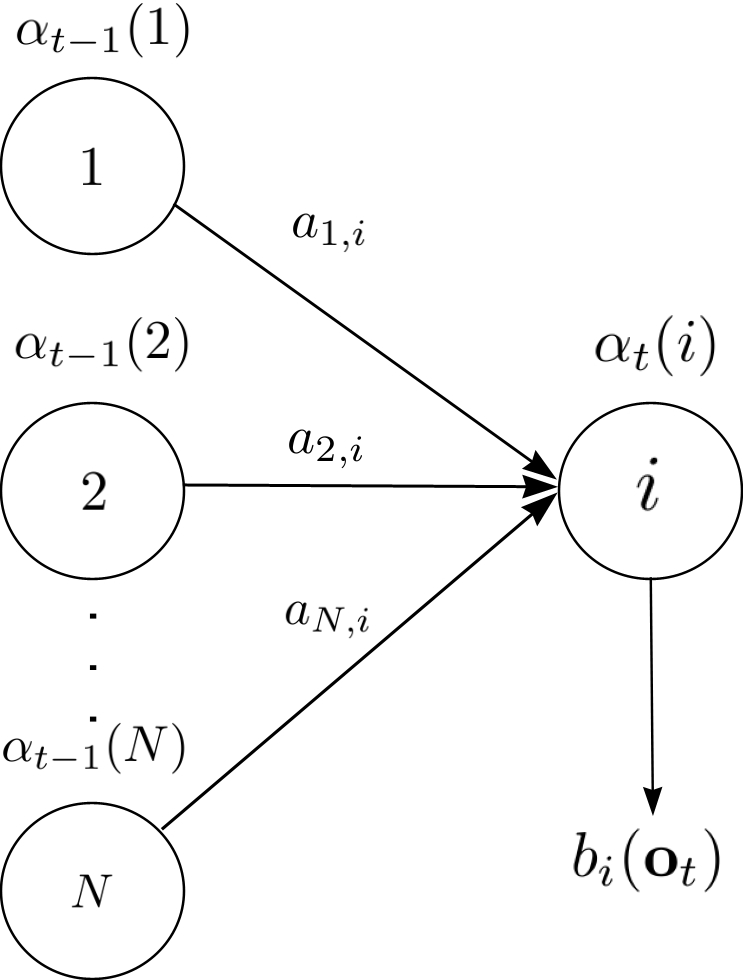
\includegraphics[width=0.25\textwidth]{forward2.jpg}
 \caption{Forward probability}
\end{figure}
The posterior probability of the observation sequence is subsequently calculated by summing over all possible end-states:
\begin{equation}
 P({\bf O}|\lambda) = \displaystyle \sum_{i = 1}^{N} \alpha_{T}(i)
\end{equation}
This holds a complexity of only $\mathcal{O}(N^{2}T)$, which is considerably less than the exponential time.
\subsection{Emmision functions}
\begin{equation}
\label{GausProbability}
 b_{j}({\bf o}_{t}) = \mathcal{N}({\bf o}_{t}; \mu_{j}, \Sigma_{j})
\end{equation}

\begin{equation}
\label{MOGprobability}
 b_{j}({\bf o}_{t}) = \displaystyle \sum_{k = 1}^K w_{k} \mathcal{N}({\bf o}_{t}; \mu_{jk}, \Sigma_{jk})
\end{equation}
Where $w_{k}$ denotes the prior probability of mixture component $k$, or weight of the mixture. 

Training the model is done by {\it Baum-Welch reestimation}, a special instance of the EM-algorithm.
\subsection{Baum-Welch reestimation}

To train the model, we need to maximise the likelihood of the parameters $\mathcal{L}(\lambda|{\bf O})$, by taking partial derivatives of every variable and setting it to zero.

To estimate $\pi_{i}$, the probability that a sequence is starting in state $i$, we divide the number of sequences starting in the state, by the total number $M$ of sequences used to train the model:
\begin{equation}
 \hat{\pi_{i}} = \frac{ \displaystyle \sum_{m = 1}^{M} \delta(q_{1}^{m} = s_{i}) }{M}
\end{equation}
Where $\delta(\cdot)$ denotes the Kronecker delta function. For the left-to-right model, the probability of entering state 1, is initialised to 1 and therefore $\pi_{i}$ will remain fixed during the whole reestimation procedure. To make the rest of the update steps more comprehensible, a set of intermediate variables is defined. First, the probability of begin in a state $i$ at timestep $t$, $P(q_{t} = s_{i} | {\bf O}, \lambda )$, which by Bayes' theorem can be written as:
\[
 (P({\bf O}|\lambda))^{-1} P({\bf O}|\lambda )P(q_{t} = s_{i}|\lambda) = 
\]
\begin{equation}
 \gamma_{t}(i) \equiv (P({\bf O}|\lambda))^{-1} \alpha_{t}(i)\beta_{t}(i) 
\end{equation}
Where normalisation constant $P({\bf O}|\lambda) = \sum_{j=1}^{N} \alpha_{t}(i)\beta_{t}(i) = \sum_{j=1}^{N} \alpha_{T}(j)$.


\[
 P(q_{t} = s_{i},q_{t+1} = s_{j}) | {\bf O}, \lambda) =
\]
\[
 \xi_{t}(i,j) \equiv (P({\bf O}|\lambda))^{-1} \alpha_{t}(i)a_{ij}b_{j}({\bf o}_{t})\beta_{t}(j)
\]
Where $\sum_{j=1}^{N} \xi_{t}(i,j) = \gamma_{t}(i)$.

With these variables defined, we can assign the derivative of the likelihood functions with respect to the model parameters an intuitive meaning. With $\xi_{t}(i,j)$ the probability of being in state $i$ and subsequently transferring to state $j$ at time $t$ and $\gamma_{t}(i)$, the total probability of being in state $i$ at time $t$, the transition probability can be updated as:
\begin{equation}
 \hat{a}_{ij} = \frac{\displaystyle \sum_{t=1}^{T-1} \xi_{t}(i,j) } {\displaystyle \sum_{t=1}^{T-1} \gamma_{t}(i) }
\end{equation}

A disadvantage about using a single Gaussian, is that for different writing styles of the same class, the Gaussian model will be trained to give the highest probability for a letter in between two instances, as illustrated by figure 3, where two different writing styles of an {\it f} are plotted in a two dimensional feature space.
\begin{figure}[ht]
  \centering
  \subfigure[Fit for single Gaussian]{
    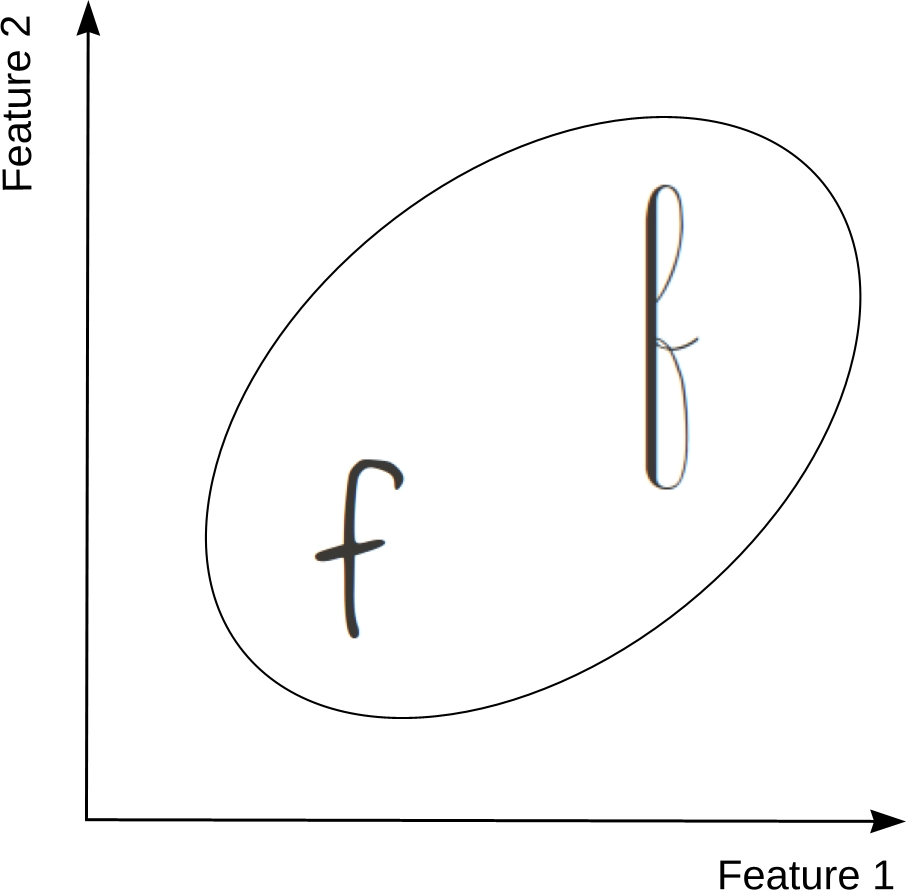
\includegraphics[scale=0.4]{single.jpg}
    \label{fig:subfig1}
  }
  \subfigure[Fit for mixture of Gaussians]{
    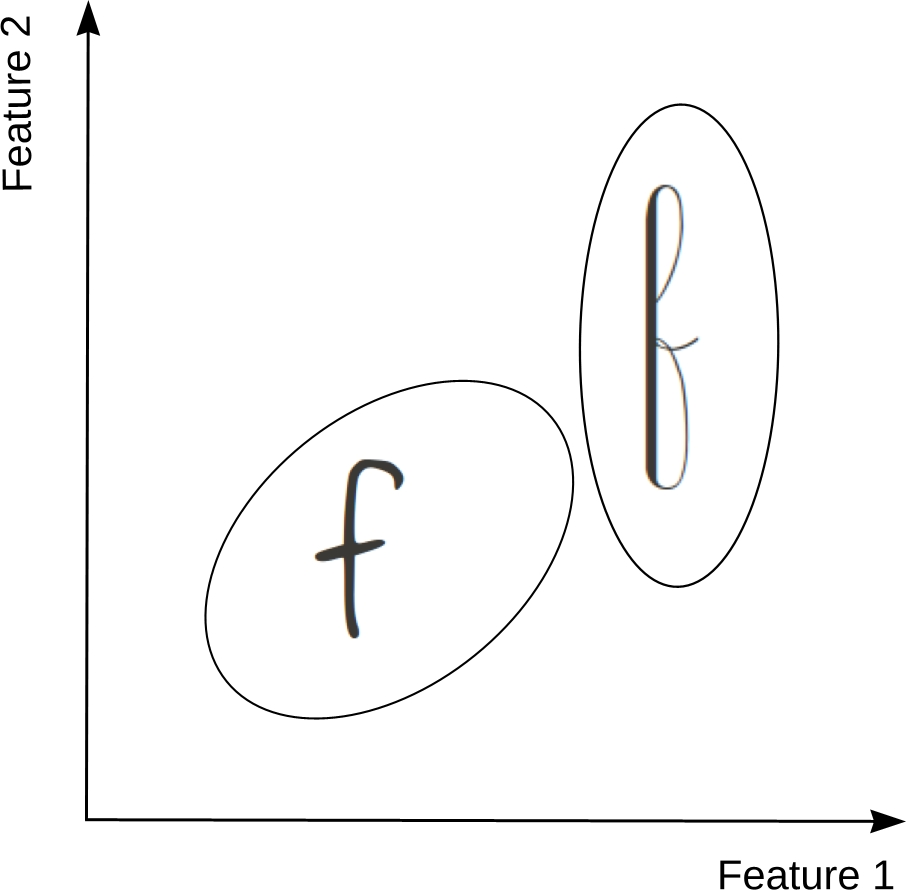
\includegraphics[scale=0.4]{gmm.jpg}
    \label{fig:subfig2}
  }
  \label{fig:subfigureExample}
  \caption[Optional caption for list of figures]{Intuition behind the Gaussian mixture model}
\end{figure}
In the case of a GMM, and aditional latent variable, the weight of each mixture component, is introduced to the system. 

\[
  P(q_{t} = s_{i}, C = k | {\bf O}, \lambda) = 
\]
\[
 P(q_{t} = s_{i}| {\bf O}, \lambda ) \frac{P({\bf o}_{t},q_{t}=s_{i},C=k|\lambda )}{ P({\bf o}_{t}, q_{t} = s_{i}| \lambda) } = 
\]
\begin{equation}
 \gamma_{t}(i,k) \equiv \gamma_{t}(i) \frac{ b_{i,k}({\bf o}_{t}) } { b_{i}({\bf o}_{t}) }
\end{equation}


\begin{equation}
 \label{updateWeightGMM}
 \hat{w}_{i,k} = \displaystyle \frac{\sum_{t=1}^{T} \gamma_{t}(i,k) }{ \sum_{t=1}^{T} \gamma_{t}(i) }
\end{equation}

\begin{equation}
 \label{updateMeanGMM}
 \hat{\bf{\mu}}_{i,k} = \displaystyle \frac{ \sum_{t=1}^{T} \gamma_{t}(i,k) {\bf o}_{t} }{ \sum_{t=1}^{T} \gamma_{t}(i,k) }
\end{equation}

\begin{equation}
 \label{updateCovarianceGMM}
 \hat{\Sigma}_{i,k} = \displaystyle \frac{ \sum_{t=1}^{T} \gamma_{t}(i,k) ({\bf o}_{t} - {\bf \mu}_{i,k})( {\bf o}_{t} - {\bf \mu}_{i,k} )^{t} }{ \sum_{t=1}^{T} \gamma_{t}(i,k) }
\end{equation}

When using a continuous observation distribution in the form of a single Gaussian or Gaussian mixture model, we have to decide upon the shape of the covariance matrix. This can either be full, diagonal or spherical/isotropic. 

\section{Experiments}
\section{Discussion}

\end{document}
